\documentclass{article}%
\usepackage[T1]{fontenc}%
\usepackage[utf8]{inputenc}%
\usepackage{lmodern}%
\usepackage{textcomp}%
\usepackage{lastpage}%
\usepackage{geometry}%
\geometry{margin=1in}%
\usepackage[utf8]{inputenc}%
\usepackage[titletoc,title]{appendix}%
\usepackage{graphicx,float}%
\usepackage{ragged2e}%
%
\title{\textbf{RELATÓRIO TÉCNICO DE SAÚDE PÚBLICA - SRAG BRASIL}}%
\date{20 de September de 2025}%
%
\begin{document}%
\normalsize%
\maketitle%
\section{Análise}%
\label{sec:Anlise}%
\subsection{Geral}%
\label{subsec:Geral}%
Nos últimos 12 meses, o número de casos de SRAG no Brasil apresentou uma tendência de aumento significativo, com um pico em maio (52.629 casos), seguido de uma redução gradual até dezembro. A maior parte do país, especialmente os estados do Centro{-}Sul, Norte e Nordeste, registrou uma incidência moderada a muito alta, enquanto regiões como Goiás, Mato Grosso do Sul e São Paulo mostraram uma tendência de queda nas últimas semanas. No entanto, estados como Amazonas, Roraima, Rio Grande do Norte e Rio Grande do Sul registraram aumento de casos, destacando a variabilidade regional.\newline%
%
A mortalidade associada à SRAG foi elevada, com 72,5\% dos óbitos relacionados à influenza A, que permaneceu como a principal causa de mortalidade. O vírus sincicial respiratório (VSR) também contribuiu significativamente para a letalidade, especialmente em crianças pequenas, cujos casos aumentaram em regiões como Amazonas e Roraima. A combinação de fatores, como a vulnerabilidade de grupos etários e a falta de vacinação em certas áreas, agravou a situação.\newline%
%
A ocupação dos leitos de Unidade de Terapia Intensiva (UTI) foi elevada durante o período de pico, especialmente em regiões com alta incidência de SRAG. A pressão sobre o sistema de saúde foi intensificada pela simultaneidade de surtos de influenza A e VSR, com alguns estados relatando dificuldades na capacidade hospitalar. A situação melhorou gradualmente no final do ano, mas permaneceu crítica em áreas com maior demanda.\newline%
%
A vacinação contra a influenza foi um dos fatores que contribuíram para a redução da letalidade em alguns estados, como São Paulo e Goiás. No entanto, a cobertura vacinal em regiões com maior incidência de SRAG, como Amazonas e Roraima, foi insuficiente, o que pode ter exacerbado a propagação da doença. A campanha de vacinação foi intensificada no final do ano, mas a eficácia depende da adesão da população e da logística de distribuição.\newline%

%
\subsection{Relação Mensal e Anual}%
\label{subsec:RelaoMensaleAnual}%
Nos últimos 30 dias, os casos de SRAG apresentaram oscilações, com um aumento em regiões como Amazonas, Roraima e Rio Grande do Sul, enquanto estados como São Paulo e Goiás registraram redução. A influenza A e o VSR continuam sendo os principais agentes etiológicos, com o VSR afetando principalmente crianças de 0 a 4 anos. A Fiocruz reforçou seus esforços de vigilância epidemiológica, incluindo a detecção de casos de gripe aviária (H5N1) confirmada em Montenegro em 2023.\newline%
%
A evolução dos casos de SRAG nos últimos 12 meses revela um padrão de aumento em maio, seguido de redução gradual, embora haja variações regionais. O pico em maio foi acompanhado por uma alta taxa de mortalidade, especialmente em áreas com baixa cobertura vacinal. A influenza A e o VSR foram responsáveis pela maioria dos casos, com o VSR afetando predominantemente crianças pequenas. A gripe aviária, confirmada em Montenegro em 2023, reforçou a necessidade de vigilância epidemiológica, enquanto a Fiocruz intensificou ações de diagnóstico e monitoramento.\newline%
%


\begin{figure}[H]%
\begin{minipage}{0.45\textwidth}%
\centering%
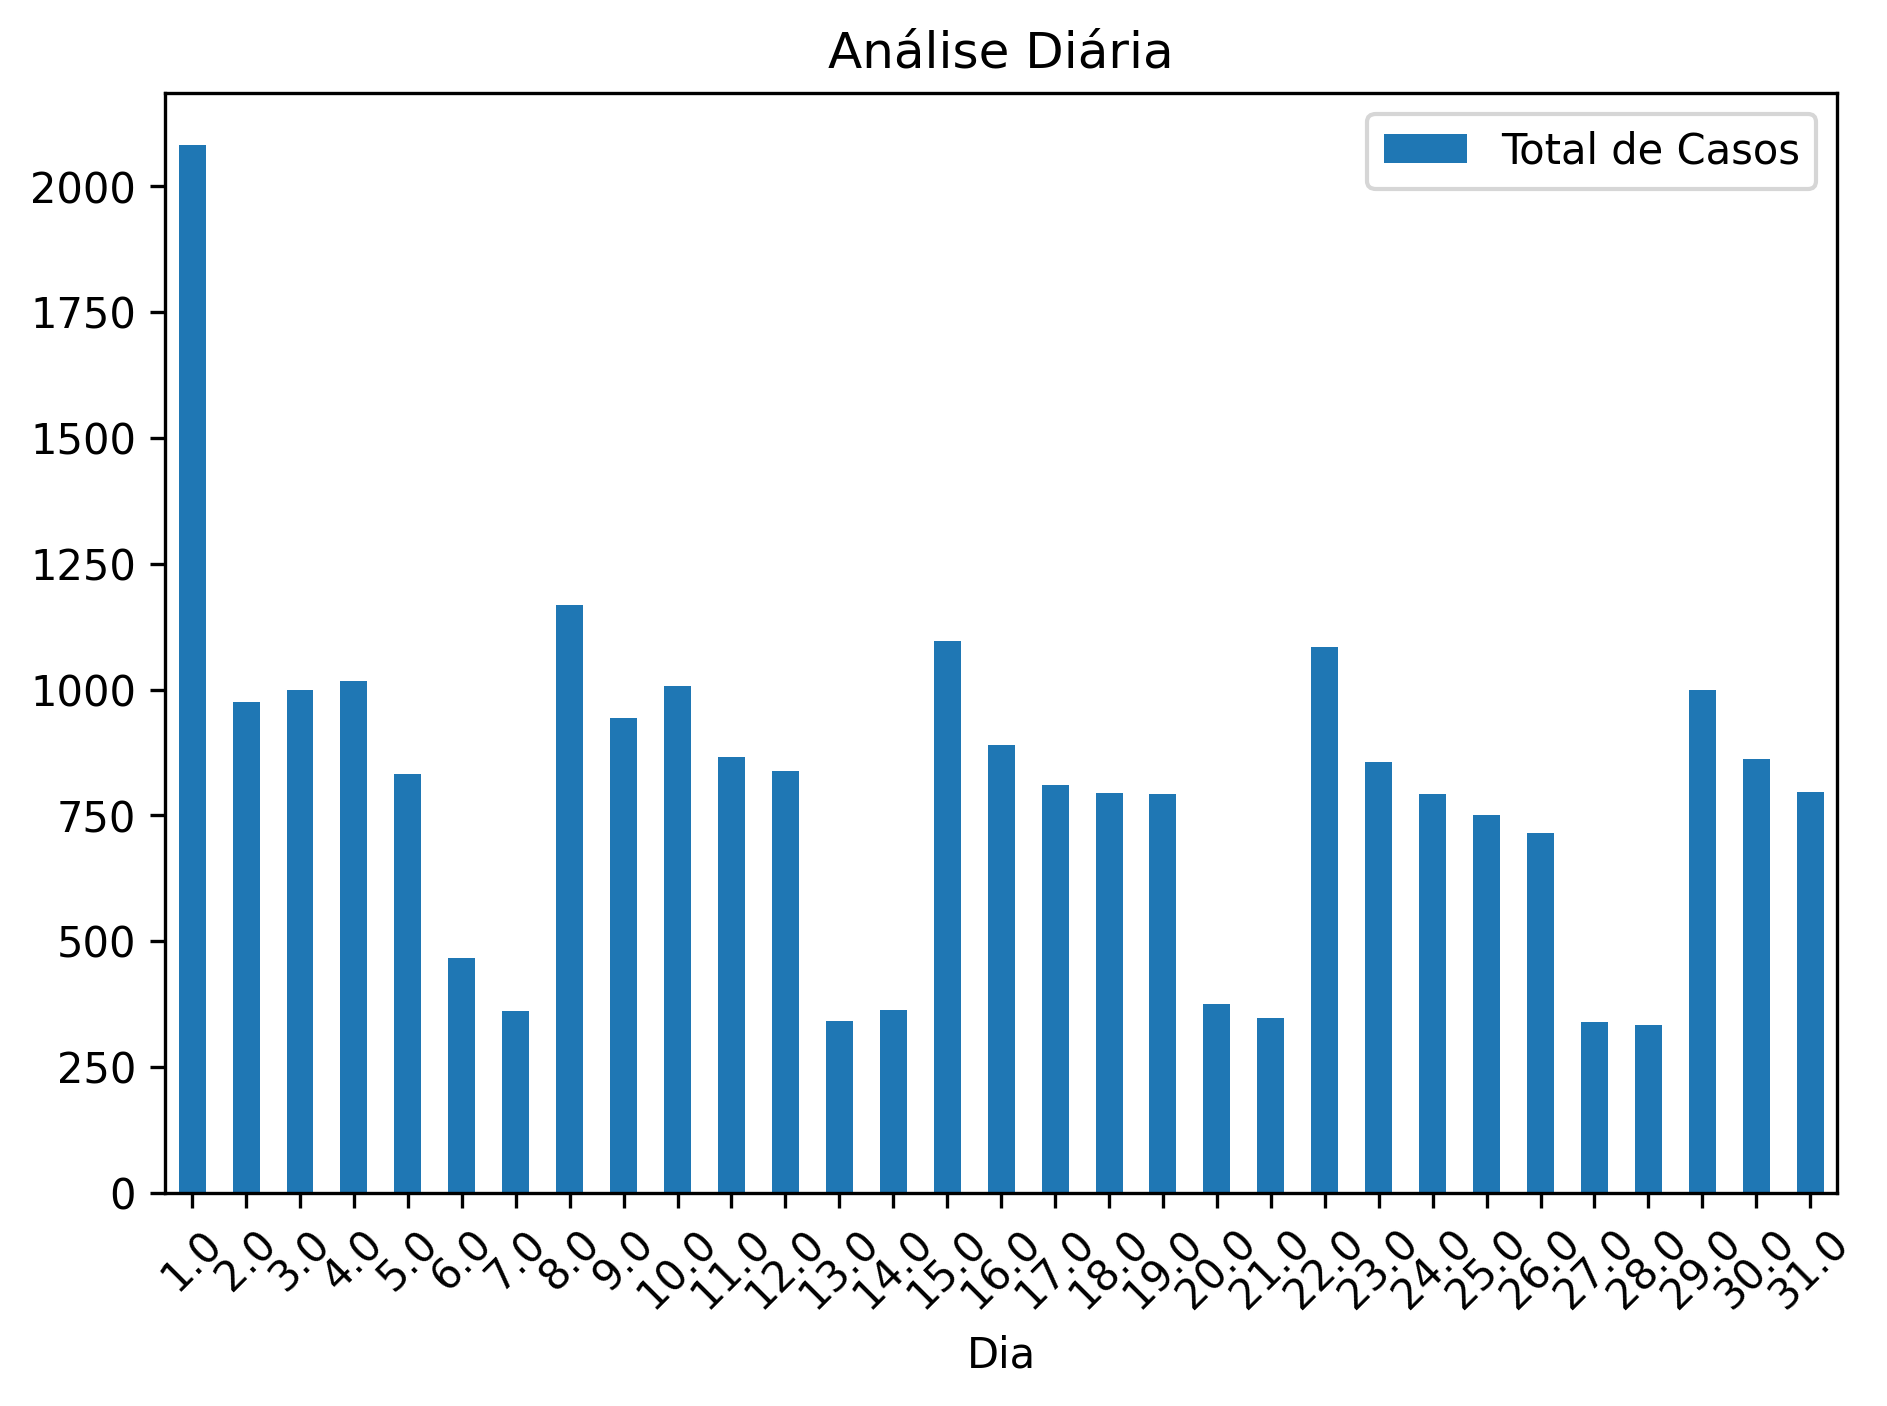
\includegraphics[width=\textwidth]{../graphics/monthly-analysis.png}%
\caption{Análise Mensal}%
\label{fig:casos-30-dias}%
\end{minipage}%
\begin{minipage}{0.45\textwidth}%
\centering%
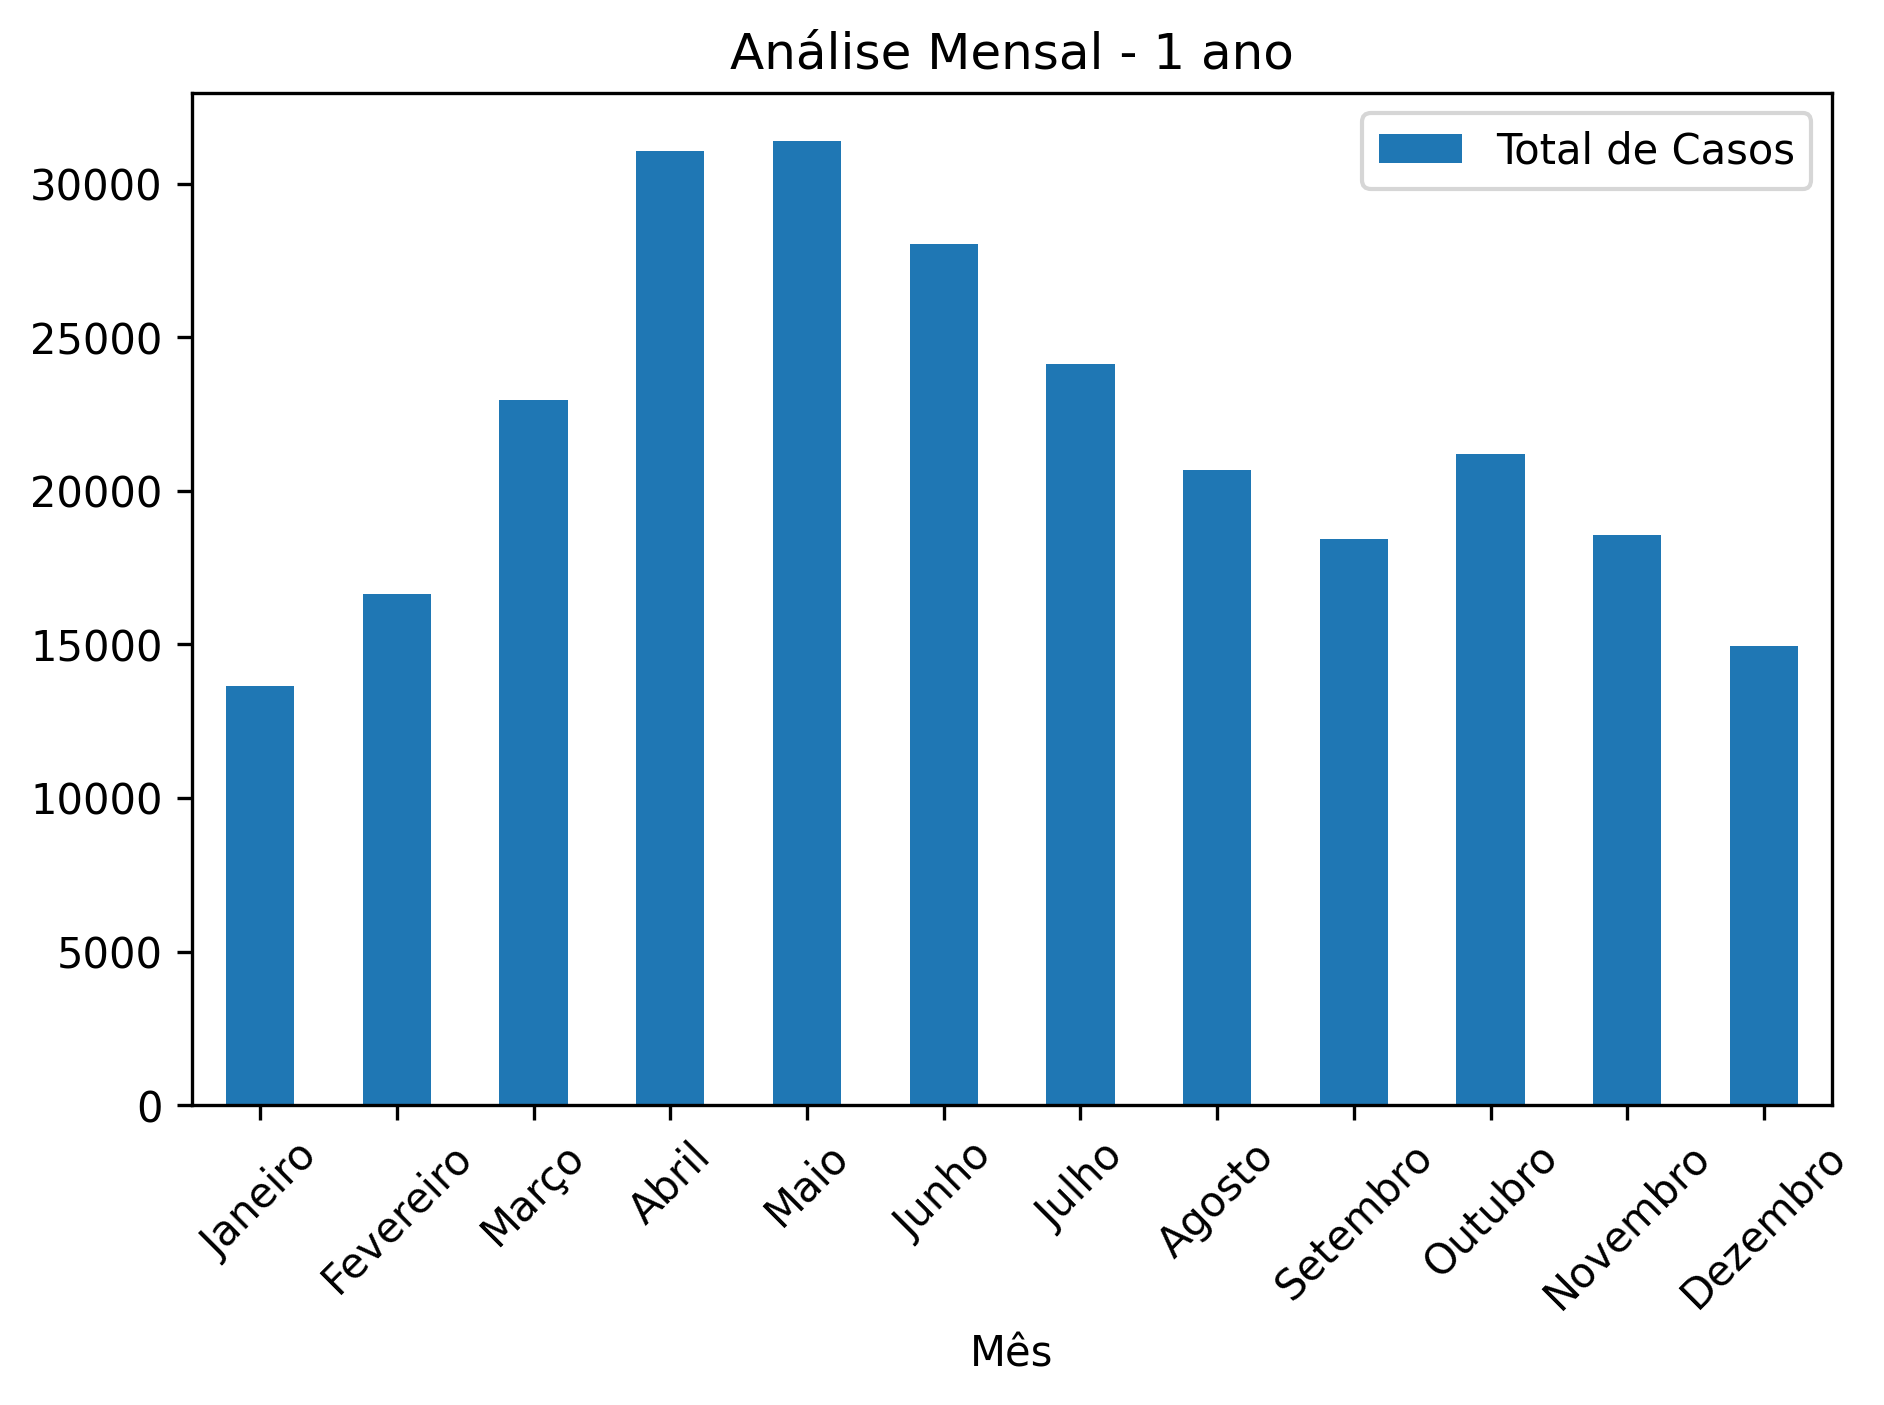
\includegraphics[width=\textwidth]{../graphics/yearly-analysis.png}%
\caption{Análise Anual}%
\label{fig:casos-12-meses}%
\end{minipage}%
\end{figure}

%
\end{document}